% CS 455, SP'22 Software Test Plan
% Software test plan template based on the template from
% https://tex.stackexchange.com/questions/42602/software-requirements-specification-with-latex
% and influenced by the IEEE 829-2008 standard
%
\documentclass[letterpaper,12pt,oneside,listof=totoc]{scrreprt}
\usepackage{listings}
\usepackage{underscore}
\usepackage{graphicx}
\usepackage{longtable}
\usepackage{float}
\usepackage[bookmarks=true]{hyperref}
\hypersetup{
    bookmarks=false,                                % show bookmarks bar
    pdftitle={Software Test Plan}, % title
%    pdfauthor={Yiannis Lazarides},                  % author
%    pdfsubject={TeX and LaTeX},                     % subject of the document
%    pdfkeywords={TeX, LaTeX, graphics, images},     % list of keywords
    colorlinks=true,                                % false: boxed links; true: colored links
    linkcolor=blue,                                 % color of internal links
    citecolor=black,                                % color of links to bibliography
    filecolor=black,                                % color of file links
    urlcolor=purple,                                % color of external links
    linktoc=page                                    % only page is linked
}%
\def\myversion{1.0 }

\date{\today}
\author{} % suppress warning, do not fill this in
\begin{document}

% we don't use \maketitle because we overide the default title page here
\begin{titlepage}
\flushright
\rule{\textwidth}{5pt}\vskip1cm
\Huge{SOFTWARE TEST PLAN}\\
\vspace{1.5cm}
for\\
\vspace{1.5cm}
Materials Ordering System\\
\vspace{1.5cm}
\LARGE{Release 1.0\\}
\vspace{1.5cm}
\LARGE{Version \myversion approved\\}
\vspace{1.5cm}
Prepared by Baxter Halder, Claire Hall, Kayla Jamar, Jennifer Olszyna\\
\vfill
\rule{\textwidth}{5pt}
\end{titlepage}

\tableofcontents
% this will be automatically created from chapters, sections, and subsections

\listoffigures
% this will be automatically created from the figure environment

\listoftables
% this will be automatically created from the table environment

\chapter*{Revision History}
% Update this table for each revision of the requirements
% Add the new content followed by a \hline

\begin{tabular}{| c | p{0.60\textwidth} | p{0.30\textwidth} |}
\hline
Date     & Description   & Revised by \\
\hline
04/11/22 & Initial draft & Data Store \\
\hline
\end{tabular}

\chapter{INTRODUCTION}

%This section introduces the following subsections, identifies the purpose of this document, and places this document in context with respect to the overall project and other documents.
The Software test plan document explains the testing activities in order to deliver a quality product.The following sections explains details of the Data Store testing process. 



\section{Scope}

%Provide a description and scope of the software and explain the goals, objectives and benefits of your project. This is the executive summary of the system and your team's subsystem.
The CS455 Monitor System software will monitor both the activity and health of all machines on a network. The system itself will be a combination of four sub-systems; Agents, a Monitoring Engine, a Data Store, and a Dashboard. The Engine and Data Store are hosted on the CS server. However, the Engine and Data Store will be portable to other server machines that run on a Unix-like OS. The Agents, installed on devices on the network, can run on both Windows and Unix-like systems. The Dashboard will display the status of the monitored machines. The Dashboard can be used on Windows or Ubuntu machines. Users will be able to view specific information such as CPU usage, memory usage, disk usage, and network usage of the monitored machines on the network from the Dashboard. This information passes through the Monitoring Engine to be validated, such as checking valid ranges for data, before being stored in the Data Store for the Dashboard to retrieve. Users will be able to view the specific machines the Agents are monitoring that are connected to the network in order to track down the cause of issues. Examples of these issues include a monitored machine being disconnected or unresponsive, a monitored machine's disk is close to or over capacity, a monitored machine's CPU usage is maxed out, which services should be running on the monitored machine that are not currently running, the network usage is less than the user expected for a monitored machine, or the monitored machine's memory usage is close to capacity. 




\section{References}
\begin{longtable}{ p{0.25\textwidth} p{0.60\textwidth} } 
   \textbf{ Standard} & \textbf{Reference }\\
    \hline
    SEI CERT & \href{https://wiki.sei.cmu.edu/confluence/display/seccode}{SEI CERT Secure Coding Practices}\\
    \hline
    Microsoft SDL & \href{https://www.microsoft.com/en-us/securityengineering/sdl/practices}{Microsoft SDL Secure Development Practices}\\
    \hline   
    SQL and PL/SQL Coding Standards  & \href{http://www.dba-oracle.com/t_plsql_best_practices_standards.htm}{PL/SQL best practice Standards tips}\\
    \hline
    Standard SQL Naming Conventions & \href{http://www.dba-oracle.com/standards_schema_object_names.htm}{Oracle naming standards tips}\\
    \hline
    JSON &  \href{https://datatracker.ietf.org/doc/html/rfc8259}{RFC 8259}\\
    \hline    
\caption{References}
\end{longtable}


%List any documents, if any, which were used as sources of %information. For example, IEEE 829-2008.

\section{System Overview}

%Provide an overview of this document and its organization.
The Software Test plan provides an organized blueprint on the process of testing the necessary requirements leading to a immaculate Data Store component. The document includes a summarized test schedule,responsibilities, and techniques used for preparing the testing trials. These trials will be assembled within the master test plan and will be be placed in certain levels based on their classification according to the integrity level scheme.

\section{Organization}
%Describe how the testing process is related to the other project processes such as requirements, management, design, quality assurance, and configuration management. Include lines of communication in the testing organization and show how they relate to the overall project organization. 
The team leader will acknowledge requirements and report progress of the project. The software engineer will proceed in developing those requirements using accurate programming and tools. Once requirements are met, the testing lead will be responsible for confirming that the requirements were encountered and efficient. If an error is detected, the testing lead will warn the following members and allow the testing engineer to record the test results and provide recommendations to improve the software. The software quality assurance engineer will be aware of each of these phases for documentation purposes of  risk and results.


\section{Master test schedule}
The first component listens to the Engine and then receives either error messages or JSON files containing information from the Agents. 
The second component is the database itself that will implemented as a MariaDB database hosted on the CS server. The database's schema is depicted in Figure~\ref{erdiagram} as an E/R diagram.
It is assumed by the Data Store that the data is valid, so once the file is received the Data Store will parse out the information contained in the file and insert it into the \textit{devices} entity or parse and insert the error message details into the \textit{error_log} entity. A database entity is a thing, person, place, unit, object or any element data should be stored in the form of properties. The Data Store's database will be comprised of two entities. \textit{devices}, and the \textit{error_log}. Each entry in the \textit{devices} entity represents a device with an Agent installed on it. 
The last component will receive confirmation from dashboard to send either queries or error messages. Error messages are processed the same way ones from the Engine are, and quires are transforms into SQL quires and processed. 
The specific test are shown below in the Master Test plan.

\begin{figure}[H]
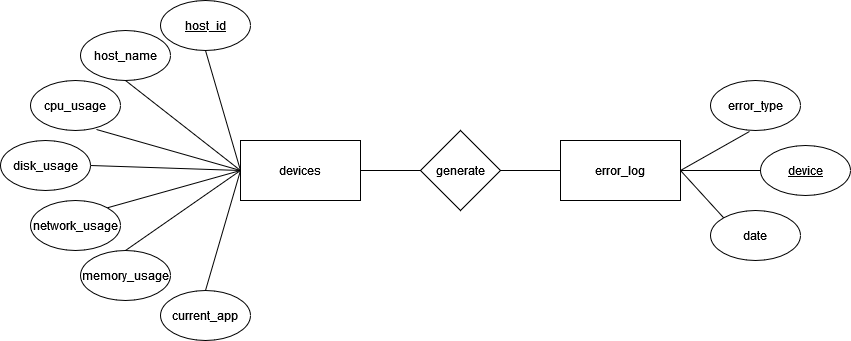
\includegraphics[scale=0.45]{Data Store Folder/er_diagram.png}
\caption{Database Design Depicted as an E/R Diagram}
\label{erdiagram}
\end{figure}


\section{Software integrity levels}
\begin{table}[H]
\centering
\caption{Software integrity levels}
\begin{tabular}{|c|c|}
\hline
Integrity level & \\
identifier      & Description \\
\hline
Level 4         & Catastrophic \\
Level 3         & Critical \\
Level 2         & Marginal \\
Level 1         & Negligible \\
\hline
\end{tabular}
\label{sils}
\end{table}




An integrity level scheme is used to provide a structured classification mechanism for denoting overall breadth and depth of testing for each testable portion of the system. Integrity levels may be applied to a variety of items including requirements, functions, classes or collections of functions, modules, subsystems, or whole systems. Table~\ref{sils} shows the software integrity level scheme that will be used to denote the minimum required testing tasks for a testable unit. Each testable unit will be assigned one of the four integrity levels shown. The required amount of testing is dictated by the level with Level 4 indicating exhaustive testing should be performed to ensure correctness and Level 1 testing indicating that basic functional is required. The scheme is drawn from the IEEE Standard for Software and System Test Document (IEEE 829-2008).




\section{Resources summary}

%Give a list or summary of the resources required to perform testing.
Functional PC's will be needed to access the following information. The PC will require a reliable server and browser for completing all tests. The standard Windows and Linux OS terminal is specifically required.Detailed information on tools,methods and metrics can be found in  \ref{Tools,techniques, methods, and metrics} table.

\section{Responsibilities}
\begin{figure}[H]
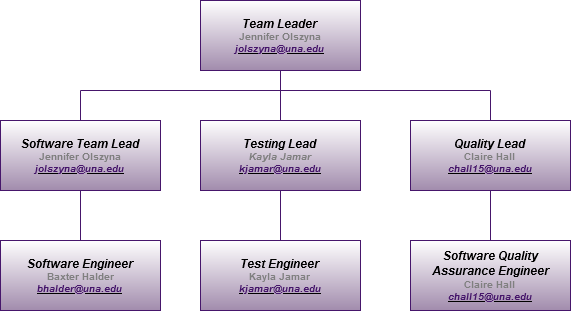
\includegraphics[scale=0.75]{Data Store Folder/org_chart.png}
\caption{Responsibility Chart}
\label{Organization Chart Listing Project}
\end{figure}

%Describe who is responsible for testing (which organizational entity) and their test-related responsibilities. You may use your org chart and refer to it.
\section{Tools, techniques, methods, and metrics}

\begin{longtable}{ p{0.15\textwidth} |  p{0.50\textwidth}} \\
\hline
\textbf{Tool} & \textbf{Purpose}  \\
\hline
XAMMP & cross-platorm web server used for testing MYSQL\\
\hline
MariaDB&  open-source GNU General Public License community-developed, commercially supported fork of the MySQL relational database management system\\
\hline
\caption{Tools, techniques, methods, and metrics}
\label{Tools,techniques, methods, and metrics}
\end{longtable}


%\chapter{MAST

%Describe the documents, hardware, software, test tools, methods, and test environment to be used in the test process.



\chapter{MASTER TEST PLAN}

\section{Level 4 test plan}
%catastrophic-exhaustive testing should be performed to ensure correctness
%requirements that are level 4
%QR7,SR01,SR06,SR27,SR02

%List the test items that are rated Level 4. All of the following subsections will be repeated for levels 3, 2, and 1 in subsequent sections.

\subsection{Traceability matrix}
\begin{longtable}{ p{0.10\textwidth} |  p{0.25\textwidth} | p{0.50\textwidth}  | p{0.50\textwidth}}
\hline
\textbf{ID} & \textbf{Requirement} & \textbf{System Component} & \textbf{Approach} \\
\hline
SR01 & Engine can create and send a network message to the Data Store & Database Tables Storing Received Messages&Black box\\
\hline
SR02 & Data store validates requests from Dashboard & Database Table Constraints&Analysis\\
\hline
SR06 & Data Store sends data to the Dashboard & SQL Queries&Analysis\\
\hline
SR27 & Data store can hold data for at least a year & Analyze Table, Check Table, Optimize Table, Repair Table, and Get Rows Count Queries&White box\\
\hline
QR7 & System can be ported to other devices & Configuration File&Analysis\\
\hline
\caption{Level 4 Matrix Table}
\label{Level 4 Matrix Table}
\end{longtable}

%Show each test case and its source (requirement's ID). The matrix links each requirements with one or more test cases. This may be a table.

%\subsection{Approach}

%List each test item and how it will be tested using the following categories:
%\begin{itemize}
%\item Black box - test cases are developed from the item specification without looking at the implementation
%\item White box - test cases are developed with knowledge of both the specification and the implementation
%\item Analysis - viewing the tested item's output is inadequate to determine if the test passed or failed because some additional computations, simulation, or other analysis is required
%\item Inspection - a static test where documentation or code is read and examined without being executed
%\end{itemize}

%NOTE: This section may be combined with the traceability matrix into a single table.

\subsection{Pass/Fail criteria}

%State the criteria used to determine if a single test case passed or failed. For example, ``Level 4 tests must successfully complete all test cases''.
Level 4 must successfully complete all test cases.

%\section{Suspension/Resumption criteria}
%  ** N/A **
% This section describe when test may be suspended and what must be done when tests are resumed.

\subsection{Test deliverables}

%List and describe the deliverables for each test case. Include how the deliverable will be recorded, tracked, and reported. This may be a table. For example, your team might use a spreadsheet to record test results, track it in your CM system, and report it via a weekly summary report.
All test results will be recorded in  excel spread sheet


% And now the level 3 test section
%critical
%requirements that are level 3
%SR13,SR14,SR15,SR16,SR17,SR28
\section{Level 3 test plan}

\subsection{Traceability matrix}
\begin{longtable}{ p{0.10\textwidth} |  p{0.25\textwidth} | p{0.50\textwidth}  | p{0.50\textwidth}}
\hline
\textbf{ID} & \textbf{Requirement} & \textbf{System Component}&\textbf{Approach} \\
\hline
SR13 & Users can view CPU usage & Device Table Storing CPU Usage, SQL Queries&White box\\
\hline
SR14 & Users can view memory usage & Device Table Storing Memory Usage, SQL Queries&White box\\
\hline
SR15 & Users can view disk usage & Device Table Storing Disk Usage, SQL Queries&White box\\
\hline
SR16 & Users can view network usage & Device Table Storing Memory Network, Queries&White box\\
\hline
SR17 & Users can view monitored services & Device Table Storing Monitored Service, SQL Queries&White box\\
\hline
SR28 & Data can be archived or removed by users & Archive Database Tables, Insert and Delete Queries&White bpx\\
\hline
\caption{Level 3 Matrix Table}
\label{Level 3 Matrix Table}
\end{longtable}

%\subsection{%Approach}

\subsection{Pass/Fail criteria}
Level 3 must successfully complete all test cases.
\subsection{Test deliverables}
All test results will be recorded in the excel spreadsheet.

% And now the level 2 test section
%marginal-
%requirements that are level 2
%SR11,SR26

\section{Level 2 test plan}

\subsection{Traceability matrix}
\begin{longtable}{ p{0.10\textwidth} |  p{0.25\textwidth} | p{0.50\textwidth} | p{0.50\textwidth} }
\hline
%modify test plan
\textbf{ID} & \textbf{Requirement} & \textbf{System Component} & \textbf{Approach}  \\
\hline
SR11 & Engine sends an error message to the Data Store when upon receiving invalid data & Error Log Table Storing Error messages & Black Box\\
\hline
SR26 & Data Store is able to scale in size & Horizontal and Vertical Scaling & White box\\
\hline
\caption{Level 2 Matrix Table}
\label{Level 2 Matrix Table}
\end{longtable}

\subsection{Approach}
Black box testing will be used to make sure data store receive the invalid data message sent from the Engine.

\subsection{Pass/Fail criteria}
Level 2 test must successfully complete all test cases

\subsection{Test deliverables}
The Error Log table will store error messages in an Excel sheet. 

% And now the level 1 test section
%negligible-small or unimportant
%testing indicating that basic functional is required.

%requirements that are level 1
%SR23,QR5


\section{Level 1 test plan}

\subsection{Traceability matrix}
\begin{longtable}{ p{0.10\textwidth} |  p{0.25\textwidth} | p{0.50\textwidth}  | p{0.50\textwidth}}
\hline
%modify test plan 
\textbf{ID} & \textbf{Requirement} & \textbf{System Component} & \textbf{Approach}\
\hline
SR23 & Data Store runs on Unix-like & CS Server (cs.csis.work) & item inspection\\
\hline
QR5 & Document and follow a coding style & SEI CERT & item inspection\\
\hline
\caption{Level 1 Matrix Table}
\label{Level 1 Matrix Table}
\end{longtable}
%\subsection{%Approach}

\subsection{Pass/Fail criteria}
Level 1 must successfully complete all test cases.
\subsection{Test deliverables}
Data Store will run on the CS server, making sure document follow a coding style.


\chapter{GENERAL}

\section{Quality assurance}

Based on the test plan matrix level, all test must be passed. If all test is not passed then a diagnostic  message will be shown, then the team will have to review what is needed for the product to pass the test. Nothing will appear or be visible to the user if the Data Store successfully runs. 


\section{Metrics}
\begin{itemize}
\item \textbf{Level-4}: Engine create and send a network to Data Store, Data store validates request from Dashboard and then sends data to the Dashboard. Data store hold data for at least a year and system can be reported to other devices. 

\item \textbf{Level-3}: User can view CPU usage,memory usage, disk usage, network usage, monitored service, and the data can be archived or removed by the user.

\item \textbf{Level-2}: Engine sends an error to the Data Store when upon receiving invalid data. Data store is able to scale in size.

\item \textbf{Level-1}: Data Store running on Unix-like and document follow a coding style.

\end{itemize}
\section{Test coverage}

The software system will require all the test coverage Level 1,2,4 uses different test coverage, but level 3 uses the same test coverage.
\end{document}
